\documentclass[SingleSpace,12pt,Journal]{Serre_ASCE}
\usepackage[dvips]{graphicx}
\usepackage[dvipsnames]{xcolor}
\usepackage{amsmath}
\usepackage{amsfonts}
\usepackage{amssymb}
\usepackage{lineno}
\usepackage{enumerate}
\usepackage{url}
\usepackage{times}
\usepackage{subfigure}
\usepackage[skip=0pt]{caption}

% TIME ON EVERY PAGE AS WELL AS THE FILE NAME
\usepackage{fancyhdr}
\usepackage{currfile}
\usepackage[us,12hr]{datetime} % `us' makes \today behave as usual in TeX/LaTeX
\fancypagestyle{plain}{
\fancyhf{}
\rfoot{\small Draft Paper \\ File Name: {\currfilename} \\ Date: {\ddmmyyyydate\today} at \currenttime}
\lfoot{Page \thepage}
\renewcommand{\headrulewidth}{0pt}}
\pagestyle{plain}

\newcommand\solidrule[1][0.25cm]{\rule[0.5ex]{#1}{1pt}}
\newcommand\dashedrule{\mbox{%
  \solidrule[2mm]\hspace{2mm}\solidrule[2mm]}}

\newcommand{\dotrule}[1]{%
	\parbox{#1}{\dotfill}} 

\makeatletter
\newcommand \Dotfill {\leavevmode \cleaders \hb@xt@ .22em{\hss .\hss }\hfill \kern \z@}
\makeatother
 
\newcommand{\Dotrule}[1]{%
   \parbox{#1}{\Dotfill}} 

\begin{document}

\title{Behaviour of the Dam-Break Problem for the Serre Equations}

\author{
Jordan~Pitt,%
\thanks{Mathematical Sciences Institute, Australian National University, Canberra, ACT 0200, Australia, E-mail: Jordan.Pitt@anu.edu.au. The work undertaken by the first author was supported financially by an Australian National University Scholarship.}
\\
Christopher~Zoppou,\footnotemark[1]%
%
% Adding a second author with the same affiliation (still using \thanks):
\\
Stephen~G.~Roberts,\footnotemark[1]
}

\maketitle

\begin{abstract}

\end{abstract}

\KeyWords{dispersive waves, conservation laws, Serre equation, finite volume method, finite difference method}

\linenumbers

%--------------------------------------------------------------------------------
\section{Introduction} \label{intro} 


%--------------------------------------------------------------------------------
\section{Serre Equations}
\label{section:Serre Equations}
The Serre equations can derived as an approximation to the full incompressible Euler equations by depth integration similar to \cite{Su-Gardener-1969-536}. They can also be seen as an asymptotic expansion of the Euler equations \cite{Bonneton-Lannes-2009-16601}. Assuming a constant hoprizontal bed the Serre equations read \cite{Guyenne-etal-2014-169}
\begin{linenomath*}
\begin{subequations}\label{eq:Serre_nonconservative_form}
\begin{gather}
\dfrac{\partial h}{\partial t} + \dfrac{\partial (uh)}{\partial x} = 0
\label{eq:Serre_continuity}
\end{gather}
\begin{gather}
\underbrace{\underbrace{\dfrac{\partial (uh)}{\partial t} + \dfrac{\partial}{\partial x} \left ( u^2h + \dfrac{gh^2}{2}\right )}_{\text{Shallow Water Wave Equations}} + \underbrace{\dfrac{\partial}{\partial x} \left (  \dfrac{h^3}{3} \left [ \dfrac{\partial u }{\partial x} \dfrac{\partial u}{\partial x} - u\dfrac{\partial^2 u}{\partial x^2}  - \dfrac{\partial^2 u}{\partial x \partial t}\right ] \right )}_{\text{Dispersion Terms}} = 0.}_{\text{Serre Equations}}
\label{eq:Serre_momentum}
\end{gather}
\end{subequations}
\end{linenomath*}
Where $u$ is the average horizontal velocity over the depth of water $h$ and $g$ is the acceleration due to gravity. 
\subsection{Conservation of mass and momentum}
The Serre equations are based on conservation of mass and momentum, thus our numerical methods should reflect this property. The total of a quantity $q$ in a system is measured by

\begin{gather}
\label{eqn:Condef}
\mathcal{C}_q(t) = \int_{-\infty}^{\infty} q\, dx
\end{gather}
so that we have for all $t$ both $\mathcal{C}_{h}(0) = \mathcal{C}_{h}(t)$ and $\mathcal{C}_{uh}(0) = \mathcal{C}_{uh}(t)$ which represents conservation of mass and momentum respectively.

\subsection{Hamiltonian}

The Serre equations admit a Hamiltonian \cite{Li-Y-2002,Hank-etal-2010-2034,Green-Naghdi-1976-237}
\begin{gather}
\label{eqn:Hamildef}
\mathcal{H}(t) = \frac{1}{2}\int_{-\infty}^{\infty} hu^2 + gh^2 + \frac{h^3}{3} \left(\frac{\partial u}{\partial x}\right)^2\, dx
\end{gather}
The Hamiltonian is such that $\mathcal{H}(t) = \mathcal{H}(0)$ for all times $t$. The Hamiltonian can be calculated numerically by partitioning the total integral into cell-wise integrals. The cell-wise integral can then be calculated by quartic interpolation utilising neighbouring cells and then applying Gaussian quadrature with $3$ points over the cell to get a sufficiently high order method, in particular this method is at least third order accurate for the $\partial u / \partial x$ term. 
%--------------------------------------------------------------------------------
\section{Direct Numerical Methods} 
\label{sec:DirNumMet}
%--------------------------------------------------------------------------------
The presence of the mixed spatial temporal derivatives in the momentum equation \eqref{eq:Serre_momentum} makes the Serre equations difficult to solve with standard numerical methods. A naive way to avoid this is to approximate \eqref{eq:Serre_momentum} by finite differences and the results of this are presented here. To facilitate this a uniform grid in space will be used with $\Delta x  = x_{i+1} - x_i$ for all $i$. Quantities evaluated at these grid points will be denoted by subscripts for example $h_i = h(x_i)$. The grid in time is also uniform and will be denoted by superscripts for example $h^n = h(t^n)$, note that $h^n$ is a function of space. 
\subsection{Finite Difference Appximation to Conservation of Momentum Equation} 
\label{subsec:FDA2conmom}
\citeN{Zoppou-etal-2017} demonstrated that an efficient numerical scheme for the Serre equations must be at least second-order accurate thus the derivatives in \eqref{eq:Serre_momentum} will be approximated by second-order finite differences. Firstly \eqref{eq:Serre_momentum} must be expanded, making use of \eqref{eq:Serre_continuity} one obtains
\begin{linenomath*}
\begin{subequations}
\begin{gather}
h\dfrac{\partial u}{\partial t} + X - h^2\frac{\partial^2 u}{\partial x \partial t} - \frac{h^3}{3}\frac{\partial^3 u}{\partial x^2 \partial t}  =0 
\label{eq:expandedu}
\end{gather}
where $X$ contains only spatial derivatives and is
\begin{gather}
X = uh\frac{\partial u}{\partial x} + gh\frac{\partial h}{\partial x} + h^2\frac{\partial u}{\partial x}\frac{\partial u}{\partial x} + \frac{h^3}{3}\frac{\partial u}{\partial x}\frac{\partial^2 u}{\partial x^2} - h^2u\frac{\partial^2 u}{\partial x^2}- \frac{h^3}{3}u\frac{\partial^3 u}{\partial x^3} .
\end{gather}
\end{subequations}
\end{linenomath*} Taking the second-order centred finite difference approximation to the spatial and temporal derivatives for \eqref{eq:expandedu} after some rearranging gives
\begin{linenomath*}
\begin{gather}
h^{n}_iu^{n+1}_i - \left(h^{n}_i\right)^2 \left(\frac{u^{n+1}_{i+1} -u^{n+1}_{i-1} }{2 \Delta x}\right) - \frac{\left(h^{n}_i\right)^3}{3}\left(\frac{u^{n+1}_{i+1} - 2u^{n+1}_{i} + u^{n+1}_{i-1} }{\Delta x^2}\right) = - Y^n_i 
\label{eq:expandedutdisc3}
\end{gather}
\end{linenomath*}
where
\begin{linenomath*}
\begin{gather*}
Y_i^n = 2\Delta tX_i^{n} - h_i^{n}u_i^{n-1} + \left(h_i^{n}\right)^2\left(\frac{u^{n-1}_{i+1} -u^{n-1}_{i-1} }{2 \Delta x}\right) + \frac{\left(h_i^{n}\right)^3}{3}\left(\frac{u^{n-1}_{i+1} - 2u^{n-1}_{i} + u^{n-1}_{i-1} }{\Delta x^2}\right) .
\label{eq:expandfactor Xp}
\end{gather*}
\end{linenomath*}
Equation \eqref{eq:expandedutdisc3} can be rearranged into a tri-diagonal matrix that updates $u$ given its current and previous values. So that
\begin{linenomath*}
\begin{gather}
\left[\begin{array}{c}
 u^{n+1}_0 \\
 \vdots \\
 u^{n+1}_m \end{array}\right]
 = A^{-1} \left[\begin{array}{c}
  -Y^n_0 \\
  \vdots \\
  -Y^n_m \end{array}\right] =: \mathcal{G}_u\left(\boldsymbol{u}^n,\boldsymbol{h}^n, \boldsymbol{u}^{n-1},\boldsymbol{h}^{n-1}, \Delta x, \Delta t \right).
\label{eq:FDcentforu}
\end{gather}
\end{linenomath*}
In particular this is an implicit numerical method for \eqref{eq:Serre_momentum}, that requires the current and previous values of $h$ and $u$.


\subsection{The Lax Wendroff Method for Conservation of Mass Equation}
\label{section:}
Because the conservation of mass equation \eqref{eq:Serre_continuity} has no mixed derivative term standard numerical techniques for conservation laws can be used. In particular the Lax-Wendroff method as done by \citeN{El-etal-2006}, here we present the method in replicable detail.

Note that \eqref{eq:Serre_continuity} is in conservative law form for $h$ where the flux is $uh$. Thus using the previously defined spatio-temporal discretisation the two step Lax-Wendroff update for $h$ is
\begin{linenomath*}
\begin{gather}
h^{n + 1/2}_{i+ 1/2} = \frac{1}{2}\left(h^{n}_{i+1} + h^{n}_i\right) - \frac{\Delta t}{2\Delta x}\left(u^n_{i+1}h^n_{i+1} - h^n_{i}u^n_{i}\right),
\end{gather}
\begin{gather}
h^{n + 1/2}_{i- 1/2} = \frac{1}{2}\left(h^{n}_{i} + h^{n}_{i-1}\right) - \frac{\Delta t}{2\Delta x}\left(u^n_{i}h^n_{i} - h^n_{i-1}u^n_{i-1}\right),
\end{gather}
\begin{gather}
h^{n+1}_i = h^{n}_i - \frac{\Delta t}{\Delta x}\left(u^{n + 1/2}_{i+ 1/2}h^{n + 1/2}_{i+ 1/2} - u^{n + 1/2}_{i- 1/2}h^{n + 1/2}_{i- 1/2}\right).
\label{eq:LW4h}
\end{gather}
\end{linenomath*}
To calculate $u^{n + 1/2}_{i \pm 1/2}$ first $u^{n+1}$ is obtained by appling $\mathcal{G}_u$ to $u^n$ then linear interpolation in both space and time gives
\begin{gather}
u^{n + 1/2}_{i+ 1/2} = \frac{u^{n+1}_{i+1} + u^{n}_{i+1} + u^{n+1}_{i} + u^{n}_{i} }{4},
\end{gather}
\begin{gather}
u^{n + 1/2}_{i- 1/2} = \frac{u^{n}_{i} + u^{n}_{i} + u^{n+1}_{i-1}+ u^{n}_{i-1} }{4}.
\end{gather}
Thus we have the following update scheme
\begin{linenomath*}
\begin{gather}
\left[ \begin{array}{l}
\boldsymbol{h}^{n+1} \\
\boldsymbol{u}^{n+1}
 \end{array}\right] = \mathcal{E}\left(\boldsymbol{u}^n,\boldsymbol{h}^n, \boldsymbol{u}^{n-1},\boldsymbol{h}^{n-1}, \Delta x, \Delta t \right). 
\end{gather}
\end{linenomath*}

%--------------------------------------------------------------------------------
\subsection{Second Order Naive Finite Difference Method}
%--------------------------------------------------------------------------------
Here we also present a completely naive method for comparative purposes, to do this we apply the procedure used above on \eqref{eq:Serre_momentum} to \eqref{eq:Serre_continuity}. Thus the derivatives were first expanded then approximated by second order centered finite differences after rearranging this to give an update formula we obtain
\begin{linenomath*}
\begin{gather}
h^{n+1}_i = h^{n-1}_i - \Delta t \left(u^{n}_{i}\frac{h^{n}_{i+1} - h^{n}_{i-1}}{\Delta x} + h^{n}_{i}\frac{u^{n}_{i+1} - u^{n}_{i-1}}{\Delta x}\right).
\end{gather}
\end{linenomath*}
Preforming this update for all $i$ will be denoted by $\mathcal{G}_h\left(\boldsymbol{u}^n,\boldsymbol{h}^n,\boldsymbol{h}^{n-1} ,\Delta x, \Delta t \right)$.
Thus we get the naive second-order centred finite difference method for the Serre equations
\begin{linenomath*}
\begin{gather}
\left.
\begin{array}{l l}
\boldsymbol{h}^{n+1}&=\mathcal{G}_h\left(\boldsymbol{u}^n,\boldsymbol{h}^n, \Delta x, \Delta t \right) \\
\boldsymbol{u}^{n+1}&=\mathcal{G}_u\left(\boldsymbol{u}^n,\boldsymbol{h}^n, \boldsymbol{u}^{n-1},\boldsymbol{h}^{n-1}, \Delta x, \Delta t \right)
\end{array} \right\rbrace \mathcal{G}\left(\boldsymbol{u}^n,\boldsymbol{h}^n, \boldsymbol{u}^{n-1},\boldsymbol{h}^{n-1}, \Delta x, \Delta t \right).
\end{gather}
\end{linenomath*}
%-------------------------------------------------------------------------------- 
\section{Conservative Form of The Serre Equations}
To overcome the aforementioned difficulty of mixed derivatives the Serre equations \eqref{eq:Serre_nonconservative_form} can be reformulated into conservative form. This is accomplished by the introduction of a new quantity \cite{Hank-etal-2010-2034,Zoppou-2014}
\begin{linenomath*}
\begin{gather}
\label{eq:Gdefinition}
G = uh - h^2 \dfrac{\partial h}{\partial x} \dfrac{\partial u}{\partial x} - \frac{h^3}{3} \dfrac{\partial^2 u}{\partial x^2}.
\end{gather}
\end{linenomath*}
Consequently, \eqref{eq:Serre_nonconservative_form} can be rewritten as
\begin{linenomath*}
\begin{subequations}
\begin{gather}
\dfrac{\partial h}{\partial t} + \dfrac{\partial (uh)}{\partial x} = 0
\label{eq:Serrecon_continuity}
\end{gather}
and
\begin{gather}
\dfrac{\partial G}{\partial t} + \dfrac{\partial}{\partial x}\left(Gu + \dfrac{gh^2}{2} - \dfrac{2h^3}{3}\dfrac{\partial u}{\partial x}\dfrac{\partial u}{\partial x}\right) = 0.
\label{eq:Serrecon_momentum}
\end{gather}
\label{eq:Serrecon}
\end{subequations}
\end{linenomath*}

\subsection{A Hybrid Finite Difference-Volume Method for Serre Equations in Conservative Form}
\label{section:hybridmethod}
%--------------------------------------------------------------------------------
The conservative form \eqref{eq:Serrecon} allows for a wider range of numerical techniques such as finite element methods \cite{Guyenne-etal-2014-169} and finite volume methods \cite{Hank-etal-2010-2034,Zoppou-2014}. In this paper the first ($\mathcal{V}_1$), second ($\mathcal{V}_2$) and third-order ($\mathcal{V}_3$) finite difference-volume methods (FDVM) of \citeN{Zoppou-etal-2017} will be used. These have been validated and their order of accuracy confirmed.

\subsection{Stability Condition} 
To ensure stability of the FDVMs the time-step $\Delta t$ must satisfy the Courant-Friedrichs-Lewy (CFL) criteria \cite{Harten-etal-1983-357}

\begin{gather}
\label{eq:CFL}
\Delta t < \frac{Cr \Delta x}{2\max \left\lbrace |\lambda| \right\rbrace}
\end{gather}

 with $0<Cr\le 1$ where $\lambda$ is the wave speed. For the Serre equations it has been demonstrated that the wave speed is bounded by the wave speed of the Shallow Water Wave equations \cite{Hank-etal-2010-2034}.

\section{Numerical Simulations}
\label{section:Numerical Simulations}
%--------------------------------------------------------------------------------
In this section the methods introduced in this paper will be validated by using them to approximate an analytic solution of the Serre equations, this will also be used to verify their order of accuracy. Then an in depth comparison of these methods for a smooth approximation to the discontinuous dam break problem will be provided to investigate the behaviour of these equations in the presence of steep gradients. This is a problem that so far has only received a proper treatment in \cite{El-etal-2006}, with other research giving only a cursory investigation into the topic. 

%--------------------------------------------------------------------------------
\section{Soliton}
\label{section:Convergence Rate}
%--------------------------------------------------------------------------------
Currently cnoidal waves are the only family of analytic solutions to the Serre equations \cite{Carter-Cienfuegos-2010-259}. Solitons are a particular instance of cnoidal waves that travel without deformation and have been used to verify the convergence rates of the described methods in this paper. 

For the Serre equations the solitons have the following form
\begin{linenomath*}
\begin{subequations}
\begin{gather}
h\left(x,t\right) = a_0 + a_1\text{sech}^2\left( \kappa\left(x - ct\right)\right),
\end{gather}
\begin{gather}
u\left(x,t\right) = c\left(1 - \dfrac{a_0}{h(x,t)} \right),
\end{gather}
\begin{gather}
\kappa = \dfrac{\sqrt{3a_1}}{2a_0 \sqrt{ a_0 + a_1}}
\end{gather}
and
\begin{gather}
c = \sqrt{g \left(a_0 + a_1\right)}
\end{gather}
\end{subequations}
\label{eq:sol}
\end{linenomath*}
where $a_0$ and $a_1$ are input parameters that determine the depth of the quiescent water and the maximum height of the soliton above that respectively. In the simulation $a_0 = 1\text{m}$, $a_1 = 0.7\text{m}$ for $x\in\left[-50\text{m},250\text{m}\right]$ and $t\in\left[0\text{s},50\text{s}\right]$. With $\Delta t = 0.5 \lambda^{-1} \Delta x$ where $\lambda = \sqrt{g \left(a_0 + a_1\right)}$ which is the maximum wave speed, this satisfies the CFL condition \eqref{eq:CFL}. 

%--------------------------------------------------------------------------------
\subsection{Results}
%--------------------------------------------------------------------------------
This numerical experiment and its results for the FDVM have been reported by \citeN{Zoppou-etal-2017}, this paper only reports the results for $\mathcal{G}$ and $\mathcal{E}$. From Figure \ref{fig:FDsolh} it can be seen that $\mathcal{G}$ and $\mathcal{E}$ accurately model the highly non-linear soliton problem reproducing the analytic solution up to graphical accuracy.

To demonstrate that in fact $\mathcal{E}$ and $\mathcal{G}$ are consistent, three measures were used. The first measures the relative distance of the numerical results for $h$ and $u$ from the analytic solution, it is defined for a general quantity $q$ and an approximation to it $q^*$ at $n$ values
\begin{gather}
L_1 = \dfrac{\sum_{i = 0}^{n} \left| q_i - q^*_i\right|}{\sum_{i = 0}^{n} \left| q_i\right|}.
\end{gather}
The second measures how well the schemes conserve a quantity $q$
\begin{gather}
C_1 = \dfrac{\left| \mathcal{C}_q(0) - \mathcal{C}_{q^*}(t_f) \right|}{\left| \mathcal{C}_q(0) \right|}
\end{gather}
where $t_f$ is the final time of the numerical experiment. For $\mathcal{C}_q(0)$ the analytic value is used while a numerical calculation is used for $\mathcal{C}_{q^*}(t_f)$ which for second-order methods is equivalent to taking the sum of all the $q^*_i$'s and then multiplying by $\Delta x$. For the Serre equations the conserved quantities are mass ($h$) and momentum ($uh$). Lastly how well the scheme conserves the Hamiltonian of the Serre equations is measured by 
\begin{gather}
H_1 = \dfrac{\left| \mathcal{H}(0) - \mathcal{H}(t_f) \right|}{\left| \mathcal{H}(0) \right|}
\end{gather}
where $t_f$ is the final time of the numerical experiment. For $\mathcal{H}(0)$ the analytic value is used while a numerical calculation based on the numerical results for $h$ and $u$ is used for $\mathcal{H}(t_f)$.
%
\begin{figure}
\centering
\subfigure[][]{\label{fig:FDsolh}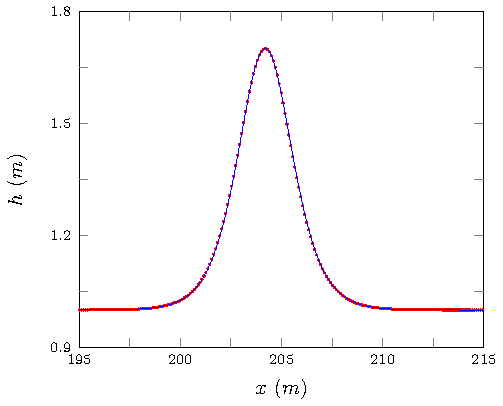
\includegraphics[width=7cm]{pics/results/soliton/ex/FDc.pdf}}
\subfigure[][]{\label{fig:FDsolhz} 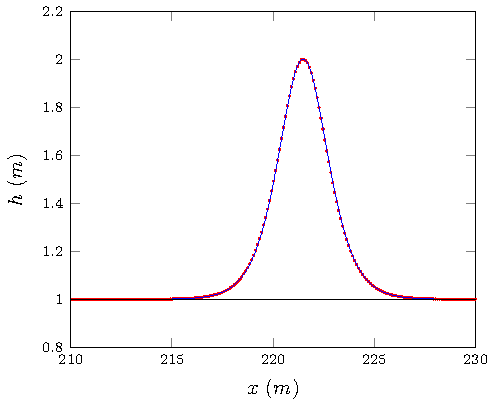
\includegraphics[width=7cm]{pics/results/soliton/ex/FDcz.pdf}}
\subfigure[][]{\label{fig:GRsolh}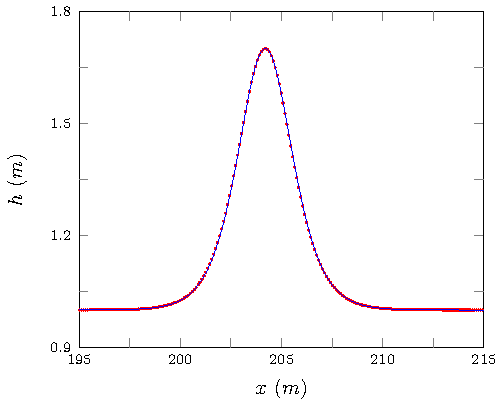
\includegraphics[width=7cm]{pics/results/soliton/ex/grim.pdf}}
\subfigure[][]{\label{fig:GRsolhz}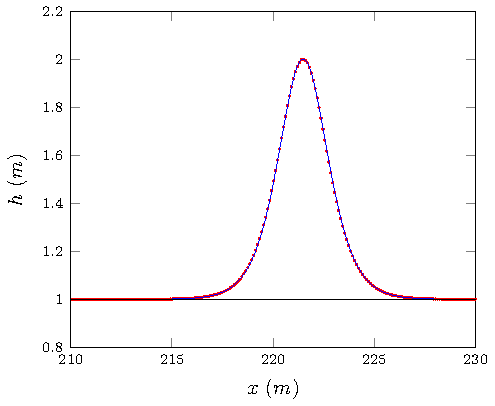
\includegraphics[width=7cm]{pics/results/soliton/ex/grimz.pdf}}
\caption{Water profile for the soliton problem \eqref{eq:sol} for $\mathcal{G}$ ((a),(b)) and $\mathcal{E}$ ((c),(d)) when $\Delta x = 10/2^{12}$ with the initial conditions ({\color{black} \solidrule}), analytic solution ({\color{blue} \solidrule}) and numerical result ({\color{red} $\bullet$}).}
\label{fig:FDMsolexp}
\end{figure}
\begin{figure}
\centering
\subfigure[][]{\label{fig:FDo2normL1}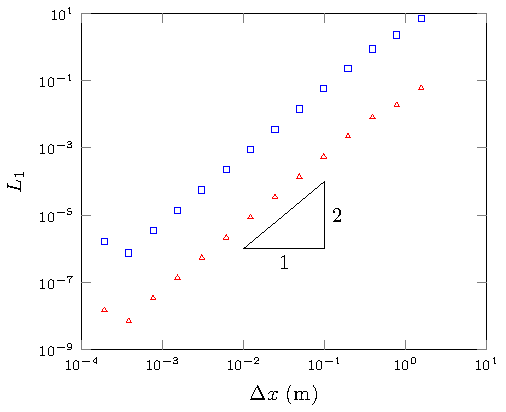
\includegraphics[width=7cm]{pics/results/soliton/L1/FDc.pdf}}
\subfigure[][]{\label{fig:FDo2Enorm}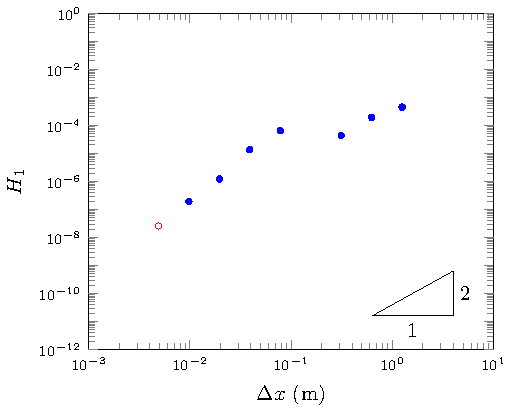
\includegraphics[width=7cm]{pics/results/soliton/H1/FDc.pdf}}
\subfigure[][]{\label{fig:grimo2normL1}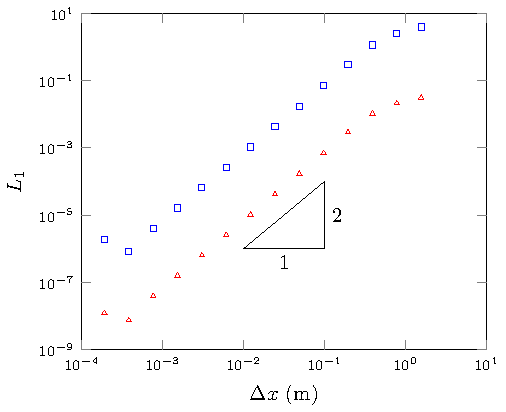
\includegraphics[width=7cm]{pics/results/soliton/L1/grim.pdf}}
\subfigure[][]{\label{fig:grimo2Enorm}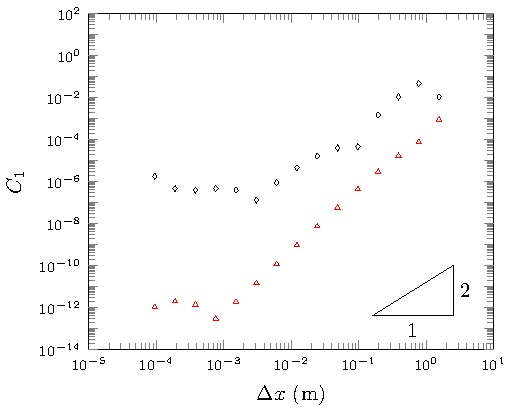
\includegraphics[width=7cm]{pics/results/soliton/H1/grim.pdf}}
\caption{On the left $L_1$ errors for $h$ ({\color{red} $\triangle$}) and $u$ ({\color{blue} $\square$}) and on the right $H_1$ ({\color{blue} $\circ$}) for the soliton problem with (a) and (b) for $\mathcal{G}$ and (c) and (d) for $\mathcal{E}$ .}
\label{fig:FDMsolnorm}
\end{figure}

\begin{figure}
\centering
\subfigure[][]{\label{fig:FDo2normC1}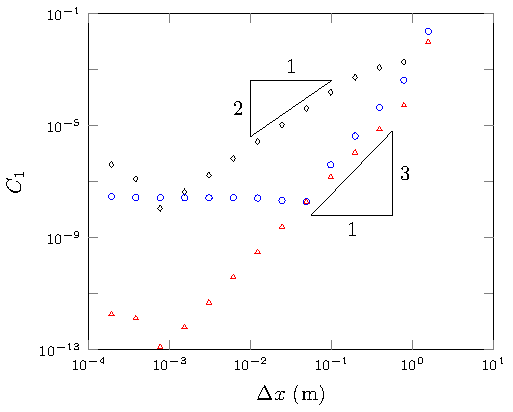
\includegraphics[width=7cm]{pics/results/soliton/C1/FDc.pdf}}
\subfigure[][]{\label{fig:grimo2normC1}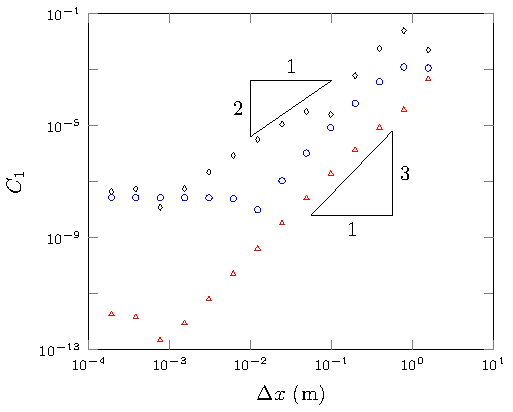
\includegraphics[width=7cm]{pics/results/soliton/C1/grim.pdf}}
\caption{$C_1$ for $h$ ({\color{red} $\triangle$}) and $uh$ ({\color{black} $\diamond$}) for numerical solutions $\mathcal{G}$ (a) and $\mathcal{E}$ (b) of the soliton problem.}
\label{fig:FDMsolnormC1}
\end{figure}
%
From Figure \ref{fig:FDMsolnorm} it can be seen that both FD methods are convergent under $L_1$ with second-order accuracy. There is however suboptimal rates of convergence for very small $\Delta x$ due to round off effects and large $\Delta x$ due to the initial conditions not being accurately represented on a coarse grid. 

From Figures \ref{fig:FDo2Enorm} and \ref{fig:grimo2Enorm} it can be seen that the FD methods conserve the Hamiltonian well and converge to the correct value of $0$ for $H_1$. Unfortunately, the point at which round off errors dominate is much earlier than for $L_1$ because $H_1$ requires more calculations than $L_1$ introducing more round off errors, although we do attain similar orders of magnitude for $L_1$ and $H_1$. 

Lastly Figure \ref{fig:FDMsolnormC1} demonstrates conservation of both mass and momentum to at least second-order for both FD schemes. Both schemes conserve mass very well with round off error dominance occurring at the same place as for $L_1$. Momentum has the appropriate order of accuracy for larger $\Delta x$ but then stagnates as $\Delta x$ decreases. This is due to the use of a finite difference method which is not necessarily conservative. Figure \ref{fig:FDMsolnormC1} however still demonstrates that these schemes are still relatively conservative and certainly there is not some drastic change in the momentum and mass in a system using these methods for smooth problems.  

All of these measures demonstrate that $\mathcal{G}$ and $\mathcal{E}$ are appropriate to solve highly non-linear problems with smooth initial conditions for the Serre equations. 

%--------------------------------------------------------------------------------
\section{Smoothed Dam-Break}
\label{section:smootheddambreak}
%--------------------------------------------------------------------------------
The discontinuous dam-break problem can be approximated smoothly using the hyperbolic tangent function. Such an approximation will be called a smoothed dam-break problem and will be defined as such
\begin{linenomath*}
\begin{subequations}
\begin{gather}
h(x,0) = h_0 + \frac{h_1 - h_0}{2}\left(1 + \tanh\left(\alpha\left(x_0 - x\right)\right)\right),
\end{gather}
\begin{gather}
u(x,0) = 0.0m/s.
\end{gather}
\end{subequations}
\label{eq:sdbi}
\end{linenomath*}
Where $\alpha$ is given and controls the width of the transition between the two dam-break heights of $h_0$ and $h_1$. We transition width is measured by taking the width of the smoothed dam-break problem inside which $90 \%$ of the transition between the two heights occurs, this will be referred to as $\beta$. $\beta$ has the following formula independent of $h_0$, $h_1$ and $x_0$
\begin{linenomath*}
\begin{gather}
\beta = \frac{2 \tanh^{-1}\left(0.9\right)}{\alpha}.
\end{gather}
\label{eq:sdbtrans}
\end{linenomath*}
\begin{figure}
\centering
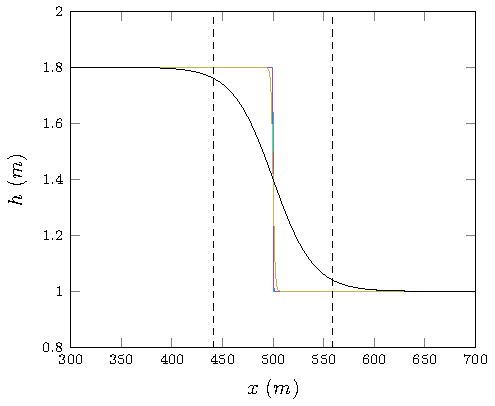
\includegraphics[width=7cm]{pics/results/SDB/init/h-figure0.pdf}
\caption{Initial conditions for the smooth dambreak problem with $\beta = 0.294$ ({\color{cyan!70!white} \solidrule}), $\beta = 1.17778$ ({\color{violet!70!white} \solidrule}), $\beta = 5.8888$ ({\color{yellow!70!black} \solidrule}) and  $\beta =117.778$ ({\color{black} \solidrule}) with reference $\beta$ interval({\color{black} \dashedrule}).}
\label{fig:dbsmoothinit}
\end{figure}
%
Figure \ref{fig:dbsmoothinit} shows the initial water profiles of smooth dam break problems with various $\beta$ values and indicates the interval in which $90\%$ of transition occurs for $\beta = 117.778$. Throughout the rest of the paper we will use $\beta$ to classify the smoothed dam break problems.

The dam break problem for the Serre equations results in the creation of an undular bore that is very similar to the analytic solution of the dam break problem for the SWWE with oscillations occurring on top \cite{Hank-etal-2010-2034}. Because of this some values from the analytic solution to the dam break problem for the SWWE will be used as a reference in this paper; these are the height ($h_2$) and velocity ($u_2$) in the shock as well as the speed of the shock front ($S_2$).  From \citeN{Wu-etal-1999-1210} we have the following equations
\begin{linenomath*}
\begin{gather}
h_2 = \frac{h_0}{2} \left[\sqrt{1 + 8 \left(\frac{2h_2}{h_2 - h_0}\frac{\sqrt{gh_1} - \sqrt{gh_2}}{\sqrt{gh_0}}\right)^2} - 1\right],
\label{eq:h2def}
\end{gather}
\end{linenomath*}
\begin{linenomath*}
\begin{gather}
u_2 = 2\left(\sqrt{gh_1} - \sqrt{gh_2}\right)
\label{eq:u2def}
\end{gather}
\end{linenomath*}
and
\begin{linenomath*}
\begin{gather}
S_2 = \frac{h_2 u_2}{h_2 - h_0}.
\label{eq:S2def}
\end{gather}
\end{linenomath*}


Undular bores for the one dimensional Serre equations were analysed by \citeN{El-etal-2006} and an expression for the amplitude ($a^+$) and speed ($S^+$) of the leading wave of a bore was given
\begin{linenomath*}
\begin{gather}
\frac{\Delta}{\left(a^+ + 1\right)^{1/4}} - \left(\frac{3}{4 -  \sqrt{a^+ + 1}}\right)^{21/10} \left(\frac{2}{1 + \sqrt{a^+ + 1}}\right)^{2/5} = 0
\label{eq:aplusdef}
\end{gather}
\end{linenomath*}
and
\begin{linenomath*}
\begin{gather}
S^+ = \sqrt{g \left(a^+ + 1\right)}
\label{eq:splusdef}
\end{gather}
\end{linenomath*}
where $\Delta = h_r / h_0$, and $h_r$ is the amplitude of the bore.

In these experiments $h_0 = 1.0m$, $h_1 = 1.8m$ and $x_0 = 500m$. This scenario replicates one presented by \citeN{El-etal-2006} and \citeN{Hank-etal-2010-2034}. The simulations were run with various values of $\Delta x$ and $\beta$. To ensure stability especially of the FD methods a very restrictive time step of $\Delta t = 0.01 \Delta x$ was chosen and for $\mathcal{V}_2$ $\theta = 1.2$. From this description the Hamiltonian at the initial time is
\begin{gather}
\label{eqn:HamilDBinit}
\mathcal{H} (0) = 10398.6 - 0.7848\times\left[\frac{2}{\alpha} \tanh\left(500 \alpha\right)\right].
\end{gather} 
Applying \eqref{eq:h2def}, \eqref{eq:u2def} and \eqref{eq:S2def} to these initial conditions results in $h_2 = 1.36898m$ , $u_2 = 1.074975$ $m/s$ and $S_2 = 3.98835$ $m/s$. For \eqref{eq:aplusdef} and \eqref{eq:splusdef} the process is a little different because $h_r \neq h_2$ but instead comes from the intersection of the Riemann invariant curve and the centred left propagating rarefaction wave curve \cite{El-etal-2006}, which results in $h_r = 1.37082$ thus $\Delta = 1.37082$,  $a^+ = 1.73998$ $m$ and $S^+ = 4.13148$ $m/s$. Of particular note is that due to the different natures of bores for the Serre and SWW equations $S^+ \neq S_2$.

%%%
%% DOWN HERE 
%%	
%%



%--------------------------------------------------------------------------------
\subsection{Results}
%--------------------------------------------------------------------------------

%Intro
We begin this study by looking into the effect of the initial steepness of the smoothed dam break problem for different $\beta$ values observing what happens as $\Delta x \rightarrow 0$ and our numerical solution better approximates the true solution of the Serre equations. To this end we use the highest order well validated model $\mathcal{V}_3$ in the following investigation. From these results we then investigate numerical results for long time scales, how the SWWE analytic values and Els whitham modulation values compare to our results and then finally present some other findings about the behaviour of our numerical solutions.

\subsubsection{effect of $\beta$}
Because the smoothing process is a non physical numerical tool we will first study its effect by decreasing $\beta$ and thus better approximating the dam break. To do this we fix a $\beta$ and then investigate the numerical solutions as $\Delta x \rightarrow 0$ and our well validated numerical methods better approximate the true solution of the equations. %We note that for a fixed $\beta$ some spatial grids will be too coarse to capture the smooth profile of the initial conditions which can cause problems for the less robust methods $\mathcal{G}$ and $\mathcal{E}$.

The first and most important observation is that there are four types of behaviour as $\Delta x \rightarrow 0$ depending on the $\beta$ and the numerical method. The four scenarios are identified by the behaviour of the solutions when $\Delta x$ is small and they correspond to different results in the literature. For brevity the only given examples of these scenarios will be the solutions of $\mathcal{V}_3$ although they also occurred for $\mathcal{E}$, $\mathcal{G}$ and $\mathcal{V}_2$.

The first behaviour which will be referred to as the non-oscillatory scenario has such smooth initial conditions that no oscillations were introduced by $t= 30s$, although given sufficient time the front steepens and an undular bore develops. An example of this behaviour can be seen in Figure \ref{fig:o3a1dxlimflatexp} for $\beta = 117.778$. Because this is a very smooth problem we observe rapid convergence with all the numerical results being graphically identical. This scenario resembles very diffusive solutions of the SWWE in that it contains only a rarefaction and a shock with no dispersive waves. 

Convergence is also present in Figure \ref{fig:o3a1dxlimmeasure} with both the $L_1$ and $H_1$ measures. However, $L_1$ has been modified to use the solution of the smallest $\Delta x$ as an approximation to the analytic solution because none are currently known. For both measures the order of accuracy is the theoretical one, with round-off errors becoming dominant for small $\Delta x$. Since $L_1$ now compares only numerical results, round-off errors result in error stagnation rather than increase. For $H_1$ it can be seen that round-off errors are dominant earlier than in $L_1$ this is because $H_1$ requires many more calculations. This suggests that this family of solutions is also a true representation of the behaviour of the Serre equations when $\beta$ is sufficiently large and in particular $\beta = 117.778$. 


\begin{figure}
\centering
\subfigure[][]{\label{fig:o3a1dxlim}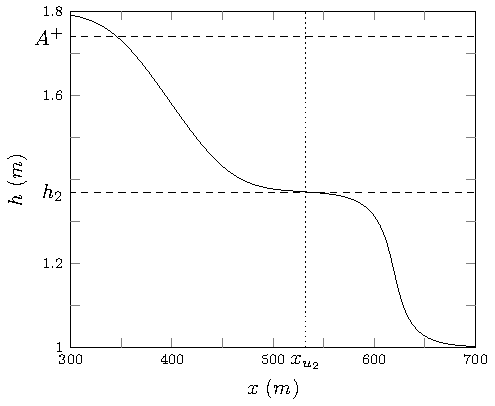
\includegraphics[width=7cm]{pics/results/SDB/numsols/alpha0.025/1-figure0.pdf}}
\caption{Numerical results of $\mathcal{V}_3$  at $t= 30s$ for the smooth dam break problem with $\beta =117.778$ for $\Delta x = 10/2^{10}$ ({\color{blue} \solidrule}), $\Delta x = 10/2^9$ ({\color{green!80!black} \solidrule}), $\Delta x = 10/2^8$ ({\color{red} \solidrule}), $\Delta x = 10/2^7$ ({\color{cyan!70!white} \solidrule}), $\Delta x = 10/2^6$ ({\color{violet!70!white} \solidrule}), $\Delta x = 10/2^5$ ({\color{yellow!70!black} \solidrule}), $\Delta x = 10/2^{4}$ ({\color{black} \solidrule}) with reference value $a^+$ ({\color{black} \dashedrule}).}
\label{fig:o3a1dxlimflatexp}
\end{figure}
%
\begin{figure}
\centering
\subfigure[][]{\label{fig:o3a1dxlimL1}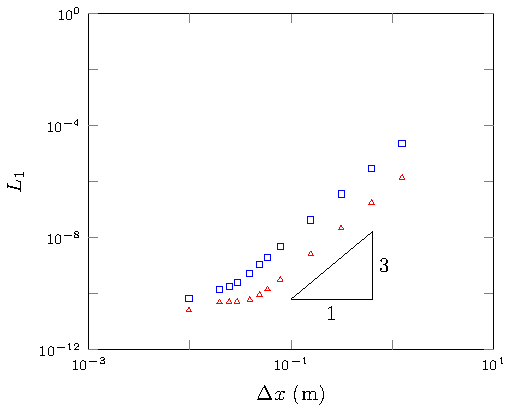
\includegraphics[width=7cm]{pics/results/SDB/Lcon/alpha0.025/1.pdf}}
\subfigure[][]{\label{fig:o3a1dxlimH}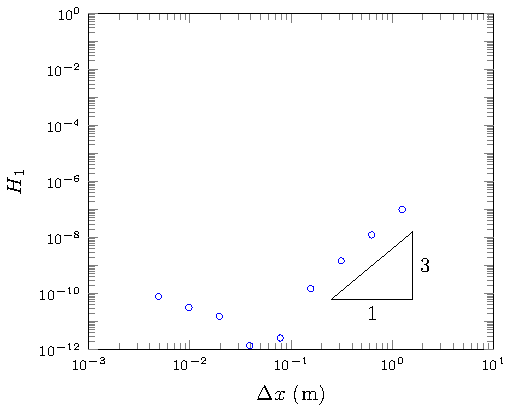
\includegraphics[width=7cm]{pics/results/SDB/Hcon/alpha0.025/1.pdf}}
\caption{$L_1$ for $h$ ({\color{red} $\triangle$}) and $u$ ({\color{blue} $\square$}) and $H_1$ ({\color{blue} $\circ$}) for $\mathcal{V}_3$'s solution for the smooth dambreak problem with $\beta =117.778$.}
\label{fig:o3a1dxlimmeasure}
\end{figure}

The second scenario will be referred to as the flat scenario due to the presence of a constant height state between the oscillations at the shock and rarefaction fan. An example of the numerical results for this scenario can be seen in Figure \ref{fig:o3a6dxlimflatexp} when $\beta = 5.8889$. This scenario corresponds to the results presented by \citeN{Hank-etal-2010-2034} and \citeN{Mitsotakis-etal-2014}. 

As $\Delta x$ decreases the solutions converge so that by $\Delta x = 10 / 2^8$ the solutions for higher $\Delta x$ are visually identical. There is also good agreement between the amplitude of the leading soliton and $a^+$ as well as the plateau height and $h_2$. Although as $\Delta x$ is decreased the plateau seems to be slightly above this value. Since this method is well validated for smooth problems and a small $\Delta x$ has been chosen this suggests that the bore from a dam break problem may differ slightly for the Serre and SWWE although they are still quite close. These results also compare well to the results in \citeN{Mitsotakis-etal-2014} who use the same $\beta$ but different $h_0$ and $h_1$. 

The measures $L_1$ and $H_1$ also demonstrate good convergence with the expected order of accuracy in the middle of the plot. Suboptimal convergence is expected for large $\Delta x$ as the problem is not sufficiently resolved to model the oscillations and so both $H_1$ and $L_1$ suffer. For small $\Delta x$ the measure $H_1$ becomes suboptimal due to round-off errors however this effect is masked by $L_1$ as a numerical solution is the base of the comparison instead of an analytic result.

\begin{figure}
\centering
\subfigure[][]{\label{fig:o3a6dxlimz1}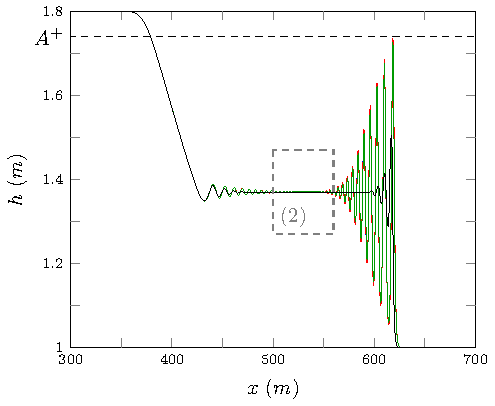
\includegraphics[width=7cm]{pics/results/SDB/numsols/alpha0.5/1-figure0.pdf}}
\subfigure[][]{\label{fig:o3a6dxlimz2}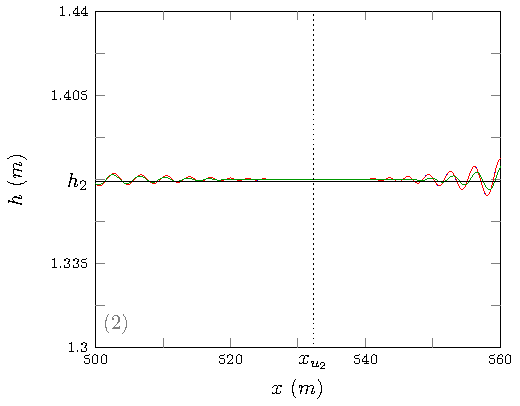
\includegraphics[width=7cm]{pics/results/SDB/numsols/alpha0.5/2-figure0.pdf}}
\caption{Numerical results of $\mathcal{V}_3$  at $t= 30s$ for the smooth dam break problem with $\beta = 5.8888$ for $\Delta x = 10/2^{10}$ ({\color{blue} \solidrule}), $\Delta x = 10/2^9$ ({\color{green!80!black} \solidrule}), $\Delta x = 10/2^8$ ({\color{red} \solidrule}), $\Delta x = 10/2^7$ ({\color{cyan!70!white} \solidrule}), $\Delta x = 10/2^6$ ({\color{violet!70!white} \solidrule}), $\Delta x = 10/2^5$ ({\color{yellow!70!black} \solidrule}), $\Delta x = 10/2^{4}$ ({\color{black} \solidrule}) with reference value $a^+$ ({\color{black} \dashedrule}).}
\label{fig:o3a6dxlimflatexp}
\end{figure}

\begin{figure}
\centering
\subfigure[][]{\label{fig:o3a2dxlimL1}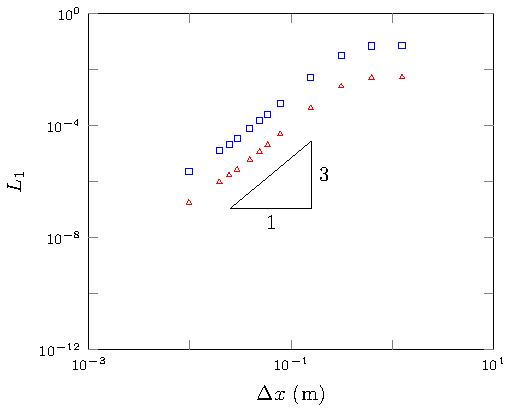
\includegraphics[width=7cm]{pics/results/SDB/Lcon/alpha0.5/1.pdf}}
\subfigure[][]{\label{fig:o3a2dxlimH}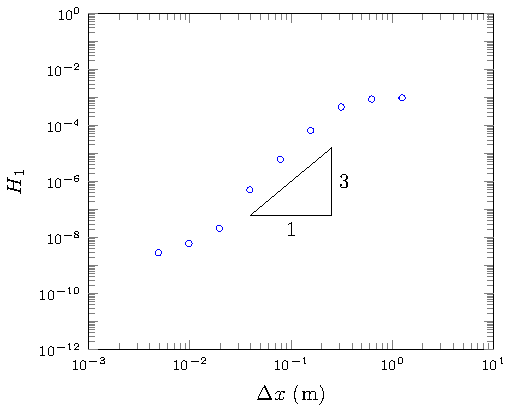
\includegraphics[width=7cm]{pics/results/SDB/Hcon/alpha0.5/1.pdf}}
\caption{$L_1$ for $h$ ({\color{red} $\triangle$}) and $u$ ({\color{blue} $\square$}) and $H_1$ ({\color{blue} $\circ$}) for $\mathcal{V}_3$'s solution for the smooth dambreak problem with $\beta = 5.8888$.}
\label{fig:o3a2dxlimmeasure}
\end{figure}

The third scenario will be referred to as the contact discontinuity \cite{El-etal-2006} scenario. The contact discontinuity scenarios main feature is that the oscillations from the rarefaction fan and the shock decay and appear to meet at a point as can be seen in Figure \ref{fig:o3a9dxlimcdexp} when $\beta = 1.1778$. All the higher order methods so far have not shown a converged solution as $\Delta x$ decreases. However, it does appear that convergence is likely with the solutions getting closer together, especially since for the smaller $\Delta x$ this problem is still smooth. These results also compare very well in terms of the lead soliton amplitude and the bore height reference values given on the plots. This scenario was observed by \citeN{El-etal-2006} for $\mathcal{E}$ and indeed we have replicated them for all the high order methods in this paper. The necessity of a $\beta$ lower than $5.8889$ to recover the `contact discontinuity' explains why \cite{Mitsotakis-etal-2014} could not replicate the results of \cite{El-etal-2006}. 

The assertion that these results are close to converged is supported by Figure \ref{fig:o3a3dxlimmeasure} for the $L^*_1$ and $H_1$ measured. As can be seen in Figure \ref{fig:o3a9dxlimz2} the final solutions have not yet even graphically converged, thus we modify $L_1$ to omit this section from $[520m,540m]$ and call this modified measure $L^*_1$. Thus $L^*_1$ demonstrates that even though this middle section has not been fully resolved we do see that there is convergence at the appropriate order outside this region. Suggesting that the effect of better resolving this contact discontinuity will only be felt locally around the contact discontinuity and not significantly change the solution away from it. $H_1$ demonstrates the appropriate order of accuracy in the Hamiltonian demonstrating that we are indeed approaching a solution to this problem as $\Delta x$ is increased. 

\begin{figure}
\centering
\subfigure[][]{\label{fig:o3a9dxlim}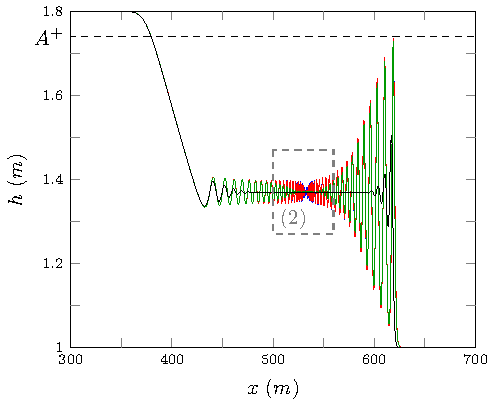
\includegraphics[width=7cm]{pics/results/SDB/numsols/alpha2.5/1-figure0.pdf}}
\subfigure[][]{\label{fig:o3a9dxlimz1}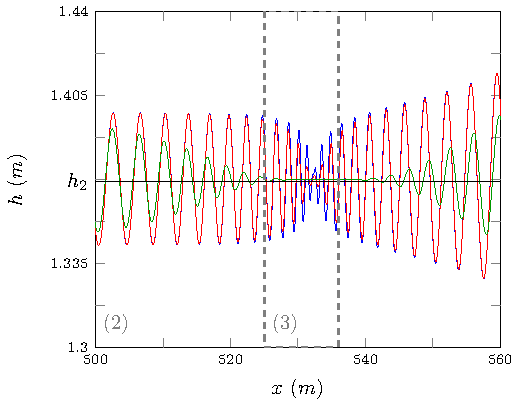
\includegraphics[width=7cm]{pics/results/SDB/numsols/alpha2.5/2-figure0.pdf}}
\subfigure[][]{\label{fig:o3a9dxlimz2}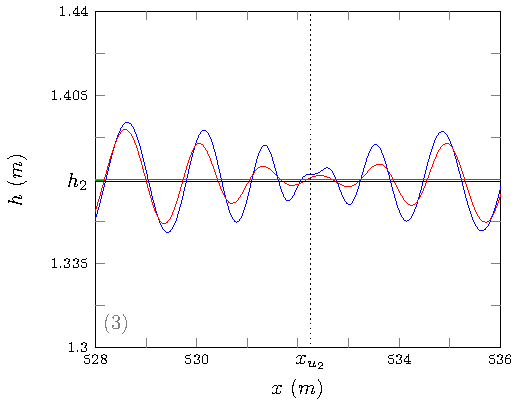
\includegraphics[width=7cm]{pics/results/SDB/numsols/alpha2.5/3-figure0.pdf}}
\caption{Numerical results of $\mathcal{V}_3$  at $t= 30s$ for the smooth dam break problem with $\beta = 1.17778$ for $\Delta x = 10/2^{10}$ ({\color{blue} \solidrule}), $\Delta x = 10/2^9$ ({\color{green!80!black} \solidrule}), $\Delta x = 10/2^8$ ({\color{red} \solidrule}), $\Delta x = 10/2^7$ ({\color{cyan!70!white} \solidrule}), $\Delta x = 10/2^6$ ({\color{violet!70!white} \solidrule}), $\Delta x = 10/2^5$ ({\color{yellow!70!black} \solidrule}), $\Delta x = 10/2^{4}$ ({\color{black} \solidrule}) with reference value $a^+$ ({\color{black} \dashedrule}).}
\label{fig:o3a9dxlimcdexp}
\end{figure}


\begin{figure}
\centering
\subfigure[][]{\label{fig:o3a3dxlimL1}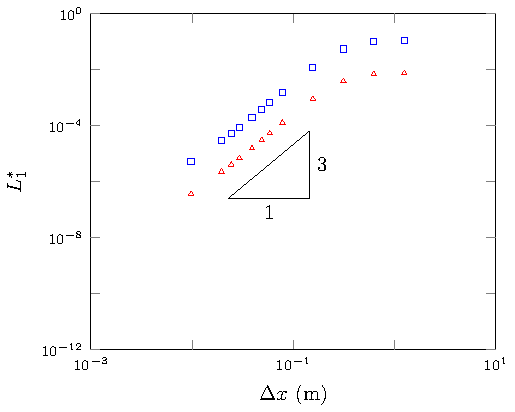
\includegraphics[width=7cm]{pics/results/SDB/Lcon/alpha2.5/1.pdf}}
\subfigure[][]{\label{fig:o3a3dxlimH}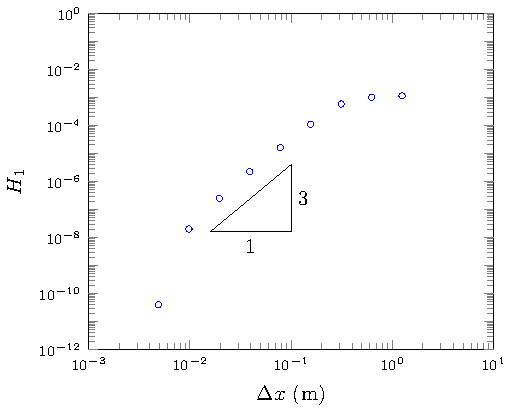
\includegraphics[width=7cm]{pics/results/SDB/Hcon/alpha2.5/1.pdf}}
\caption{$L^*_1$ for $h$ ({\color{red} $\triangle$}) and $u$ ({\color{blue} $\square$}) and $H_1$ ({\color{blue} $\circ$}) for $\mathcal{V}_3$'s solution for the smooth dambreak problem with $\beta = 1.17778$.}
\label{fig:o3a3dxlimmeasure}
\end{figure}


The fourth scenario will be referred to as the bump scenario due to the oscillations no longer decaying down towards a point but rather growing around the contact discontinuity forming a bump as can be seen in Figure \ref{fig:o3a20dxlimcdexp} for $\beta = 0.294$. This behaviour has hitherto not been published and is certainly not an expected result. 

This scenario is even further from graphical convergence in $\Delta x$ around the contact discontinuity than the previous scenario as can be seen in Figure \ref{fig:o3a20dxlimcdexp}. $L^*_1$ demonstrates good convergence outside this middle region as can be seen in Figure \ref{fig:o3a4dxlimmeasure}. $H_1$ also converges but only has the appropriate order of accuracy in the last few $\Delta x$ points. This suggests that to properly resolve this scenario requires smaller grids or higher-order schemes. Because, convergence is not assured by these numerical results there is the possibility that the wave amplitudes around the contact discontinuity could explode. This however has not been observed, with numerical results where $\beta = 0.00294$ and $\Delta x = 10.0/ 2^{10}m = 0.009765625m$ at which point the initial conditions are basically a discontinuous dam break showing an increase but not an explosion in amplitude.

\begin{figure}
\centering
\subfigure[][]{\label{fig:o3a20dxlim}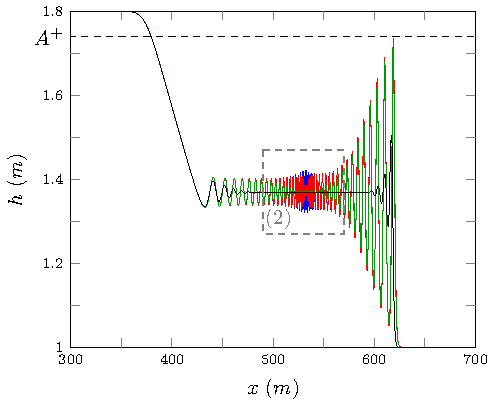
\includegraphics[width=7cm]{pics/results/SDB/numsols/alpha10/1-figure0.pdf}}
\subfigure[][]{\label{fig:o3a20dxlimz1}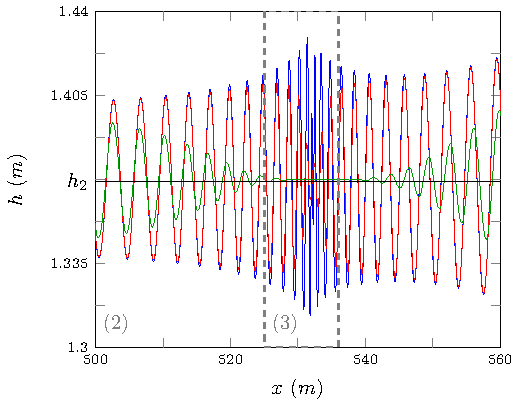
\includegraphics[width=7cm]{pics/results/SDB/numsols/alpha10/2-figure0.pdf}}
\subfigure[][]{\label{fig:o3a20dxlimz2}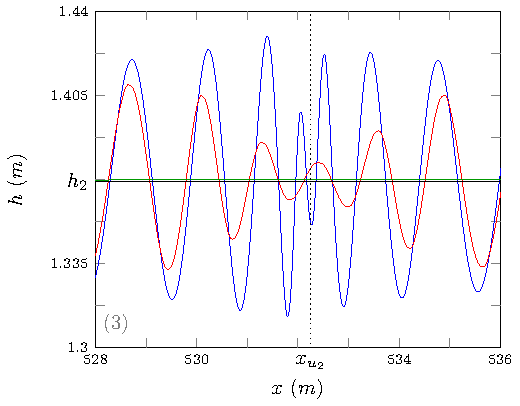
\includegraphics[width=7cm]{pics/results/SDB/numsols/alpha10/3-figure0.pdf}}
\caption{Numerical results of $\mathcal{V}_3$  at $t= 30s$ for the smooth dam break problem with $\beta = 0.294$ for $\Delta x = 10/2^{10}$ ({\color{blue} \solidrule}), $\Delta x = 10/2^9$ ({\color{green!80!black} \solidrule}), $\Delta x = 10/2^8$ ({\color{red} \solidrule}), $\Delta x = 10/2^7$ ({\color{cyan!70!white} \solidrule}), $\Delta x = 10/2^6$ ({\color{violet!70!white} \solidrule}), $\Delta x = 10/2^5$ ({\color{yellow!70!black} \solidrule}), $\Delta x = 10/2^{4}$ ({\color{black} \solidrule}) with reference value $a^+$ ({\color{black} \dashedrule}).}
\label{fig:o3a20dxlimcdexp}
\end{figure}

\begin{figure}
\centering
\subfigure[][]{\label{fig:o3a4dxlimL1}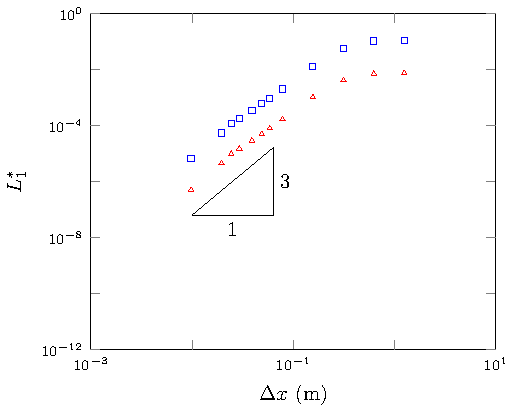
\includegraphics[width=7cm]{pics/results/SDB/Lcon/alpha10/1.pdf}}
\subfigure[][]{\label{fig:o3a4dxlimH}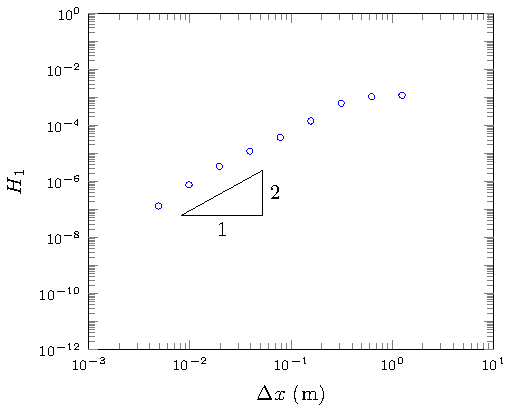
\includegraphics[width=7cm]{pics/results/SDB/Hcon/alpha10/1.pdf}}
\caption{$L^*_1$ for $h$ ({\color{red} $\triangle$}) and $u$ ({\color{blue} $\square$}) and $H_1$ ({\color{blue} $\circ$}) for $\mathcal{V}_3$'s solution for the smooth dambreak problem with $\beta = 0.294$.}
\label{fig:o3a4dxlimmeasure}
\end{figure}

% % % % % % % % % % % % % % % % % % % % MOST WORK DOWN HERE!!!! % % % % % % % % % % % % % % % % % % % % % %
% % % % % % % % % % % % % % % % % % % % % %% % % % % % % % % % % % % % % % % % % % % %% % % % % % % % % % %
% % % % % % % % % % % % % % % % % % % % % %% % % % % % % % % % % % % % % % % % % % % %% % % % % % % % % % %
% % % % % % % % % % % % % % % % % % % % % %% % % % % % % % % % % % % % % % % % % % % %% % % % % % % % % % %
% % % % % % % % % % % % % % % % % % % % % %% % % % % % % % % % % % % % % % % % % % % %% % % % % % % % % % %
% % % % % % % % % % % % % % % % % % % % % %% % % % % % % % % % % % % % % % % % % % % %% % % % % % % % % % %

%smoothing for El as well
%add S_2

Since this result is unexpected and not as supported as the contact discontinuity scenario in the literature \cite{El-etal-2006,Gurevich-Meshcherkin-1984-1277}. The first check should be different numerical methods such as $\mathcal{G}$ and $\mathcal{E}$ to test if some numerical effect from the reformulation of the Serre equations or the elliptic solver are the cause. For comparison all methods discussed in this paper are applied to the same initial conditions and grid resolutions as above are plotted in Figure \ref{fig:MODlim}. The first observation is that $\mathcal{V}_1$ has not recovered this behaviour. This is because as noted by \citeN{Zoppou-etal-2017}, $\mathcal{V}_1$ is very diffusive, dampening these oscillations. To resolve such behaviour for $\mathcal{V}_1$ would require very small $\Delta x$ and as such we have not seen this behaviour yet. The diffusivity of the first-order scheme is the reason why \citeN{Hank-etal-2010-2034} could not replicate the results of \citeN{El-etal-2006} with reasonable $\Delta x$. Secondly, all high order methods recover this bump behaviour and disagree only in the region around the contact discontinuity. The main difference in the oscillations is their phase and amplitude with the dispersive FD methods resulting in larger waves than the diffusive FDVM. 

Dispersive methods decrease oscillation amplitude and number as $\Delta x$ is decreased as can be seen in Figure \ref{fig:FDa6lim}. Since $\mathcal{V}_3$ is diffusive as in Figure \ref{fig:o3a20dxlimcdexp} the true analytic solution should then exist between $\mathcal{V}_3$ and $\mathcal{G}$, which is a bounded bump around the contact discontinuity. Finally it can be seen that $\mathcal{V}_2$ and $\mathcal{V}_3$ are similar. This is because as noted by \citeN{Zoppou-etal-2017} $\mathcal{V}_3$ is not a substantially better method than $\mathcal{V}_2$ and so their results are going to be quite similar. $\mathcal{G}$ well approximates the Serre equations, although the FDVM are still preferred by the authors due to robustness and conservation of quantities as can be seen in Figure \ref{fig:FDMsolnormC1}. Figure \ref{fig:o3a4dxHallsign} demonstrates that the $\mathcal{V}_i$ schemes result in $\mathcal{H}(30s) < \mathcal{H}(0s)$ so energy is only lost where as $\mathcal{G}$ and $\mathcal{E}$ can gain energy and are therefore undesirable.

\begin{figure}
\centering
\subfigure[][]{\label{fig:MODh}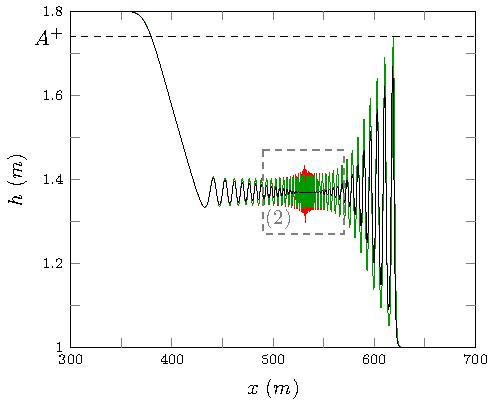
\includegraphics[width=7cm]{pics/results/SDB/numsols/modelcomppalpha10dx10/1-figure0.pdf}}
\subfigure[][]{\label{fig:MODh1}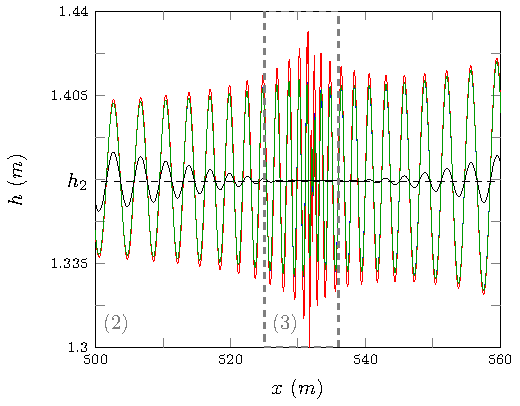
\includegraphics[width=7cm]{pics/results/SDB/numsols/modelcomppalpha10dx10/2-figure0.pdf}}
\subfigure[][]{\label{fig:MODh2}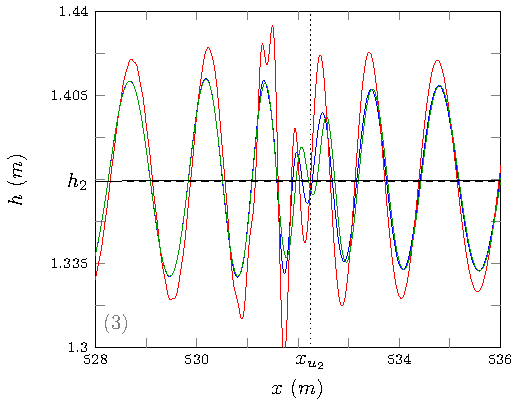
\includegraphics[width=7cm]{pics/results/SDB/numsols/modelcomppalpha10dx10/4-figure0.pdf}}
\caption{Numerical results for the smooth dam break problem with $\beta = 0.294$ and $\Delta x = 10/2^{10}$
for $\mathcal{G}$ ({\color{red} \solidrule}), $\mathcal{E}$ ({\color{cyan!70!white} \solidrule}), $\mathcal{V}_3$ ({\color{violet!70!white} \solidrule}), $\mathcal{V}_2$ ({\color{yellow!70!black} \solidrule}) and $\mathcal{V}_1$ ({\color{black} \solidrule}) with reference value $a^+$ ({\color{black} \dashedrule}).}
\label{fig:MODlim}
\end{figure}

\begin{figure}
\centering
\subfigure[][]{\label{fig:o3a4dxH1propFDVM}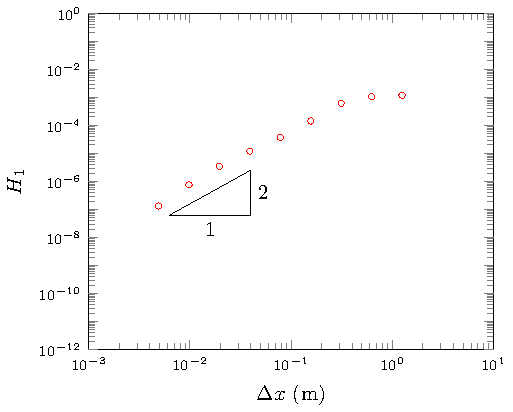
\includegraphics[width=7cm]{pics/results/SDB/Hcon/alpha10signs/o3.pdf}}
\subfigure[][]{\label{fig:o3a4dxH1propFD}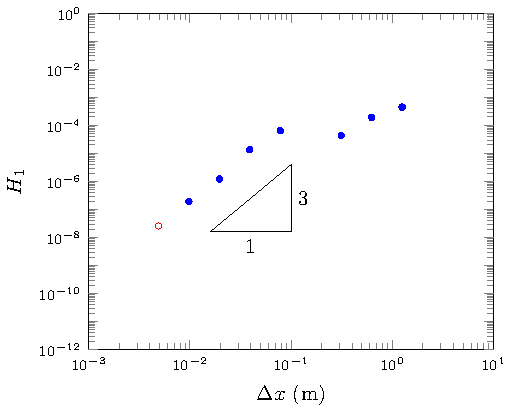
\includegraphics[width=7cm]{pics/results/SDB/Hcon/alpha10signs/FDc.pdf}}
\caption{$H_1$ for $\mathcal{V}_3$ (a) and $\mathcal{G}$'s (b) solution for the smooth dambreak problem at $t = 30s$ with $\beta = 0.294$ demonstrating when $\mathcal{H}(0s) \ge \mathcal{H}(30s)$ ({\color{red} $\circ$}) and $\mathcal{H}(0s) < \mathcal{H}(30s)$ ({\color{blue} $\bullet$}).}
\label{fig:o3a4dxHallsign}
\end{figure}



\begin{figure}
\centering
\subfigure[][]{\label{fig:FDa6h}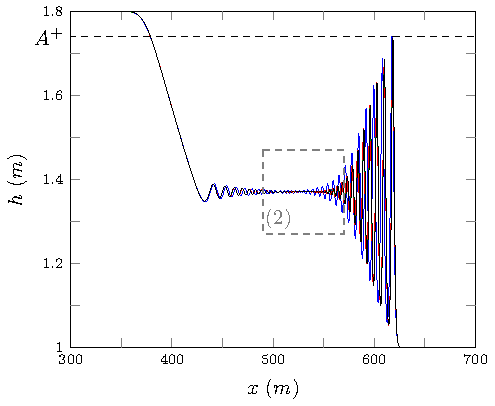
\includegraphics[width=7cm]{pics/results/SDB/numsols/FDcalpha0.5/1-figure0.pdf}}
\subfigure[][]{\label{fig:FDa6hz}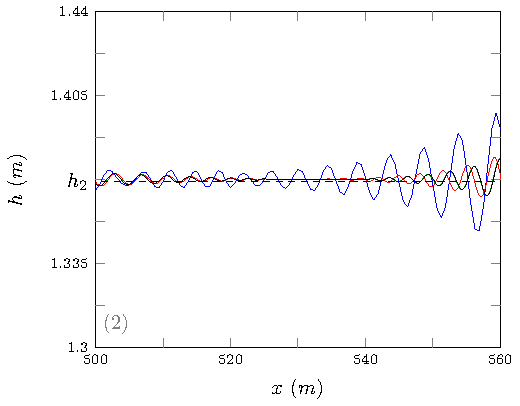
\includegraphics[width=7cm]{pics/results/SDB/numsols/FDcalpha0.5/2-figure0.pdf}}
\caption{Numerical results of $\mathcal{G}$  at $t= 30s$ for the smooth dam break problem with $\beta = 5.8888$ for $\Delta x = 10/2^{4}$ ({\color{blue} \solidrule}), $\Delta x = 10/2^5$ ({\color{green!80!black} \solidrule}), $\Delta x = 10/2^6$ ({\color{red} \solidrule}), $\Delta x = 10/2^7$ ({\color{cyan!70!white} \solidrule}), $\Delta x = 10/2^8$ ({\color{violet!70!white} \solidrule}), $\Delta x = 10/2^9$ ({\color{yellow!70!black} \solidrule}), $\Delta x = 10/2^{10}$ ({\color{black} \solidrule}) with reference value $a^+$ ({\color{black} \dashedrule}).}
\label{fig:FDa6lim}
\end{figure}


There is still the possibility that these solutions are caused by some numerical phenomena such as these methods not properly handling contact discontinuities, more research into this topic should be undertaken. However, the agreement of all the discussed methods of sufficiently high order indicates that these results are representative of actual solutions of the smoothed dam break problem with low $\beta$ for the Serre equations. Lastly we replicated this scenario with $\mathcal{E}$ using a similar order of magnitude for $\Delta x$ as \citeN{El-etal-2006}. The absence of a bump scenario in their findings suggests that either their numerical method differs from $\mathcal{E}$ or there has been smoothing of the initial conditions, both of which are absent from the paper. This concludes the explaination of how our results fit in with the current literature and now the following section of this paper will be concerned with some further numerical investigation into these results. 



%--------------------------------------------------------------------------------
\subsubsection{Long time}\label{subsubsec:LT}
%--------------------------------------------------------------------------------
The first test of these results will be of its evolution through time, thus an experiment was run with the same parameters on a larger domain with $x \in [-900m, 1800m]$ for $t \in [0,300s]$. The results for $\beta = 0.294$ and $\Delta x = 10/2^{9}$ at $t = 300s$ are presented in Figure \ref{fig:FVlonga20}. For this problem these parameters result in the bump scenario as can be seen in Figure \ref{fig:o3a20dxlimcdexp}, however after sufficient time we can see that this bump has decayed back into a flat scenario although there are still small oscillations present in the middle region. 

We also observe that the values $S^+$ and $a^+$ have not been perfectly replicated with the numerical solution giving larger values than the analytic ones derived by \citeN{El-etal-2006} although these results are close. We also note that as above the bore heights for the Serre and SWWE appear to be slightly different.

To observe the evolution of the water profile the numerical solution has been shifted by $u_2  \times t$ in Figure \ref{fig:FVlongcemt500} to give a dam break that is essentially motionless with respect to the contact discontinuity. It can be seen that at $t =30s$ the solution is in the bump scenario but as time progresses the centre region has decayed into the contact discontinuity scenario by $t=100s$ and then into the flat scenario observed at $t=200s$ and $t=300s$. This could be a property of the solution Serre equations after sufficient time or due to the accumulation of numerical diffusion with Figure \ref{fig:FVcomplonga20} demonstrating that over this timespan we are not close to convergence of the numerical results.    

\begin{figure}
\centering
\subfigure[][]{\label{fig:FVlonga20h}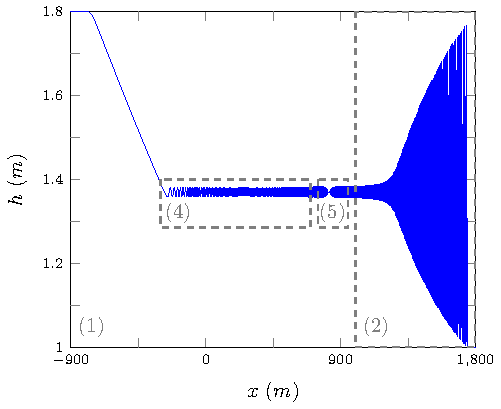
\includegraphics[width=7cm]{pics/results/SDB/numsols/300s/h0t300s.pdf}}
\subfigure[][]{\label{fig:FVlonga20hf}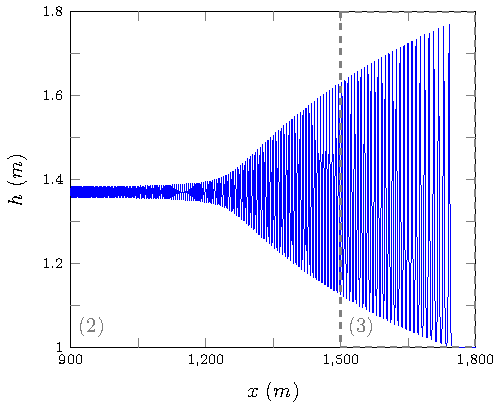
\includegraphics[width=7cm]{pics/results/SDB/numsols/300s/h1t300s.pdf}}
\subfigure[][]{\label{fig:FVlonga20hb}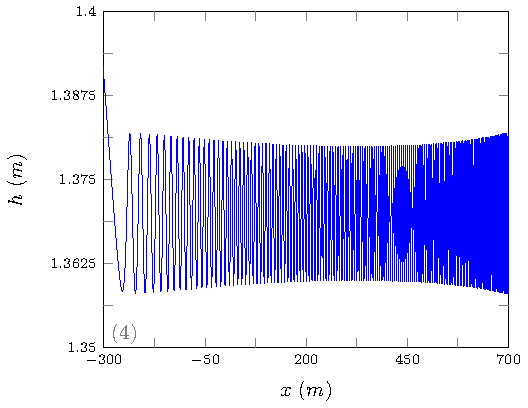
\includegraphics[width=7cm]{pics/results/SDB/numsols/300s/h2t300s.pdf}}
\subfigure[][]{\label{fig:FVlonga20hz}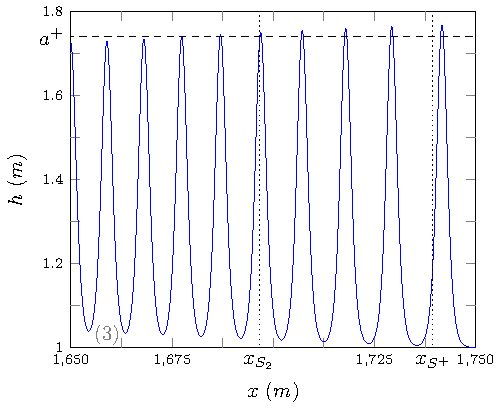
\includegraphics[width=7cm]{pics/results/SDB/numsols/300s/h4t300s.pdf}}
\subfigure[][]{\label{fig:FVlonga20hz}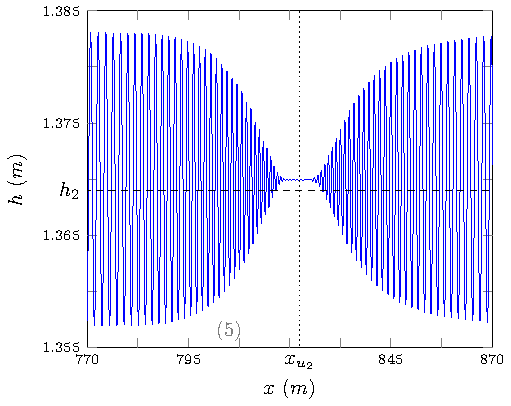
\includegraphics[width=7cm]{pics/results/SDB/numsols/300s/h3t300s.pdf}}
\caption{Smooth dam break problem at $t=300s$ for $\mathcal{V}_3$ with $\beta = 0.294$ for $\Delta x = 10/2^{9}$ ({\color{blue} \solidrule}) with reference values  $a^+$ ({\color{black} \dashedrule}) ((a), (b), (d)), $S^+$ ({\color{black} \dotrule{0.04\textwidth}}) (d), $S_2$ ({\color{black} \Dotrule{0.04\textwidth}}) (d), $h_2$ ({\color{black} \dashedrule}) (e) and $x_2$ ({\color{black} \dotrule{0.04\textwidth}}) (e).}
\label{fig:FVlonga20}
\end{figure}

\begin{figure}
\centering
\subfigure[][]{\label{fig:FVlonga20a}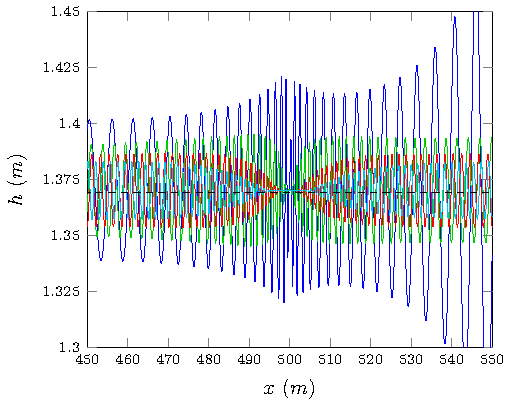
\includegraphics[width=7cm]{pics/results/SDB/numsols/300s/difftimescenteredat500m.pdf}}
\caption{Water profile shifted by $u_2 \times t$ for the numerical solution of the smoothed dam break with $\mathcal{V}_3$, $\beta = 0.294$ and $\Delta x = 10/2^{9}$ at $t=30s$ ({\color{blue} \solidrule}), $t=100s$ ({\color{green!80!black} \solidrule}), $t=200s$ ({\color{red} \solidrule}) and $t=300s$ ({\color{cyan!70!white} \solidrule}).}
\label{fig:FVlongcemt500}
\end{figure}


%coarsefinecomparison
\begin{figure}
\centering
\subfigure[][]{\label{fig:FVcomplonga20h}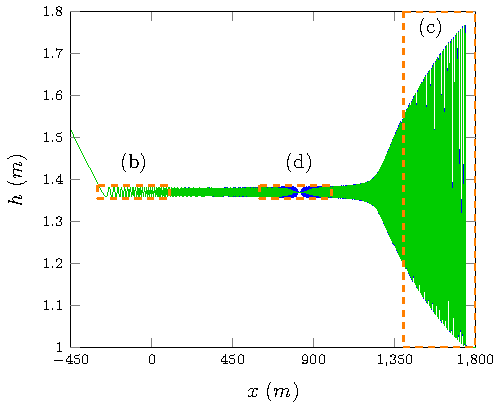
\includegraphics[width=7cm]{pics/results/SDB/numsols/300s/CF0t300.pdf}}
\subfigure[][]{\label{fig:FVcomplonga20hf}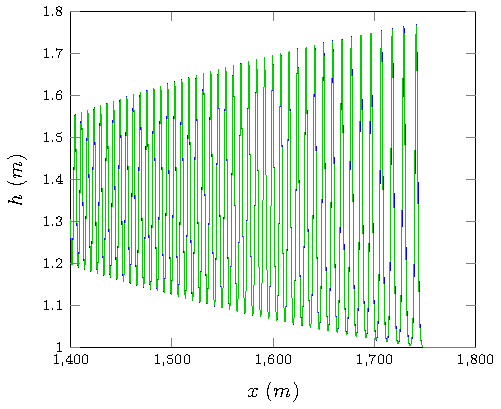
\includegraphics[width=7cm]{pics/results/SDB/numsols/300s/CF2t300.pdf}}
\subfigure[][]{\label{fig:FVcomplonga20hb}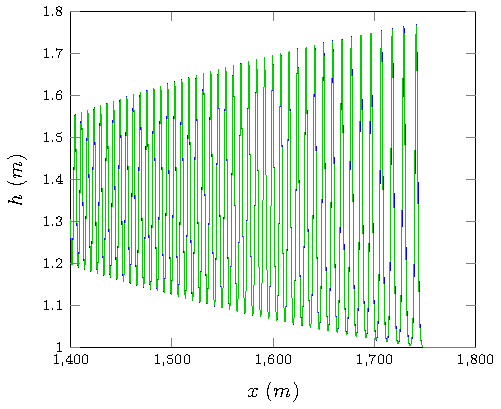
\includegraphics[width=7cm]{pics/results/SDB/numsols/300s/CF2t300.pdf}}
\subfigure[][]{\label{fig:FVcomplonga20hz}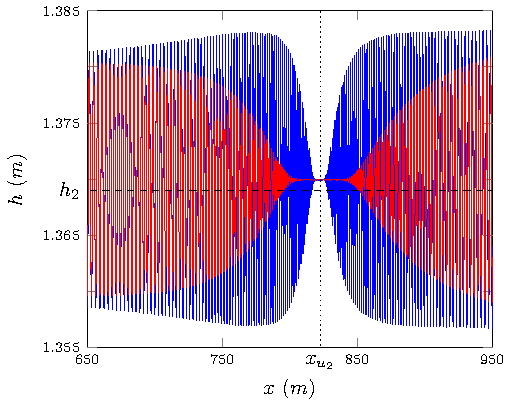
\includegraphics[width=7cm]{pics/results/SDB/numsols/300s/CF3t300.pdf}}
\caption{Smooth dam break problem at $t=300s$ for $\mathcal{V}_3$ with $\beta = 0.294$ for $\Delta x = 10/2^{9}$ ({\color{blue} \solidrule}) and $\Delta x = 10/2^{8}$ ({\color{green!80!black} \solidrule})  with reference values $h_2$ ({\color{black} \dashedrule})(d) and $x_2$ ({\color{black} \dotrule{0.04\textwidth}}) (d).}
\label{fig:FVcomplonga20}
\end{figure}

\subsubsection{SWWE comparison}
Since the SWWE have been used as a guide for the mean behaviour of the solution of the Serre equations in the literature \cite{Hank-etal-2010-2034,Dutykh-2014-315} we would like the investigate how useful they are. 
%cd speed
We begin by studying the speed of the contact discontinuity which should travel at the mean bore velocity \cite{Gurevich-Meshcherkin-1984-1277}. Since as stated before there are analytic solutions for these values for the SWWE, the numerical results can be compared to this. To investigate this $h_1$ was varied to allow for different aspect ratios and thus different bore speeds. The results are plotted in Figure \ref{fig:CDspeed} from which it is quite clear that this discontinuity does in fact travel at the bore speed for a range of aspect ratios. 
\begin{figure}
	\centering
	\subfigure[][]{\label{fig:CDspeed1}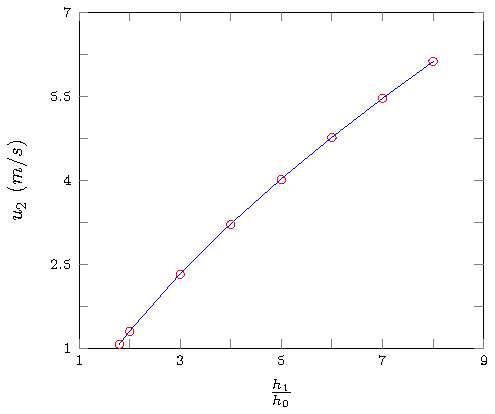
\includegraphics[width=7cm]{pics/results/SDB/CDspeed/speed.pdf}}
	\caption{$u_2$ ({\color{blue} \solidrule}) and speed of the contact discontinuity ({\color{red} $\circ$})  for $\mathcal{V}_3$ solution of the various smooth dam break problems with $\beta = 0.2944$ and $\Delta x = 10/2^{9}$ at $t=100s$.}
	\label{fig:CDspeed}
\end{figure}

%uh comparison
To further demonstrate the SWWE solution as a useful guide for mean behaviour we plot $h - h_2$ and $u - u_2$ for the smoothed dam break problem with $\beta = 0.2944$ and $\Delta x = \frac{10}{2^9}$ in Figure \ref{fig:UHSWWcomp30sall} for $t= 30s$ and Figure \ref{fig:UHSWWcomp30sall} for $t= 300s$. From this we can see that over short time spans both $h_2$ and $u_2$ are good approximations to the mean behaviour of the fluid with both plots oscillating around $0$. However after sufficient time we see that the mean velocity and height of the fluid has diverged slightly from the SWW equation values $h_2$ and $u_2$. With $h_2$ being an underestimate and $u_2$ being an overestimate. From Figure \ref{fig:FVlonga20} it can also be seen that $S_2$ underestimates the speed of the bore front.

\begin{figure}
	\centering
	\subfigure[][]{\label{fig:UHcomp1}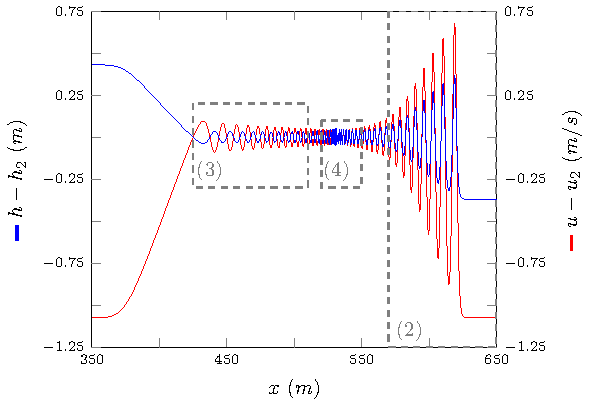
\includegraphics[width=7cm]{pics/results/SDB/numsols/SWWCOMP/30s/0.pdf}}
	\subfigure[][]{\label{fig:UHcomp2}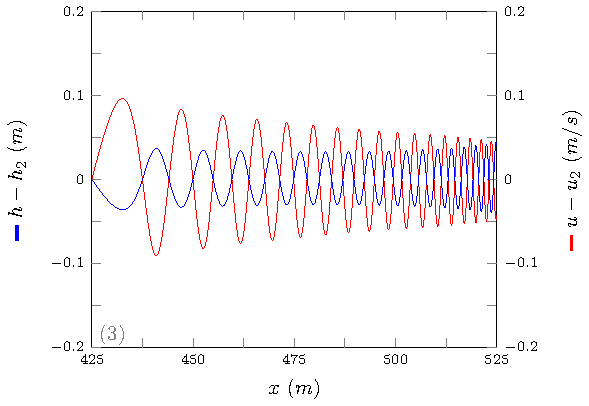
\includegraphics[width=7cm]{pics/results/SDB/numsols/SWWCOMP/30s/1.pdf}}
	\subfigure[][]{\label{fig:UHcomp3}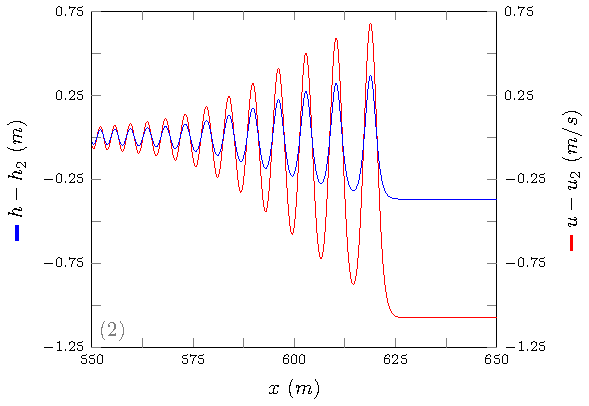
\includegraphics[width=7cm]{pics/results/SDB/numsols/SWWCOMP/30s/2.pdf}}
	\subfigure[][]{\label{fig:UHcomp4}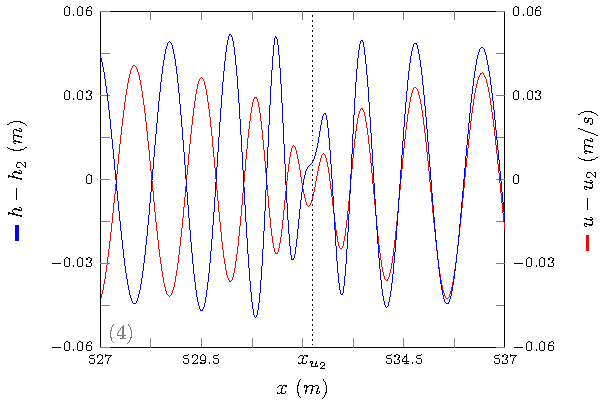
\includegraphics[width=7cm]{pics/results/SDB/numsols/SWWCOMP/30s/3.pdf}}
	\caption{$h - h_2$ ({\color{blue} \solidrule}) and $u - u_2$ ({\color{green!80!black} \solidrule}) for $\mathcal{V}_3$ solution of the smooth dam break with $\beta = 0.2944$ and $\Delta x = 10/2^{9}$ at $t=30s$.}
	\label{fig:UHSWWcomp30sall}
\end{figure}

\begin{figure}
	\centering
	\subfigure[][]{\label{fig:UH300comp1}\includegraphics[width=7cm]{pics/results/SDB/numsols/SWWCOMP/300s/0.pdf}}
	\subfigure[][]{\label{fig:UH300comp2}\includegraphics[width=7cm]{pics/results/SDB/numsols/SWWCOMP/300s/1.pdf}}
	\subfigure[][]{\label{fig:UH300comp3}\includegraphics[width=7cm]{pics/results/SDB/numsols/SWWCOMP/300s/2.pdf}}
	\subfigure[][]{\label{fig:UH300comp4}\includegraphics[width=7cm]{pics/results/SDB/numsols/SWWCOMP/300s/3.pdf}}
	\caption{$h - h_2$ ({\color{blue} \solidrule}) and $u - u_2$ ({\color{green!80!black} \solidrule}) for $\mathcal{V}_3$ solution of the smooth dam break with $\beta = 0.2944$ and $\Delta x = 10/2^{9}$ at $t=300s$.}
	\label{fig:UHSWWcomp300sall}
\end{figure}

From Figure \ref{fig:UHcomp2} and Figure \ref{fig:UHcomp4} it can also be seen that to the left of the contact discontinuity $u$ and $h$ are antiphase. While Figure \ref{fig:UHcomp3} and Figure \ref{fig:UHcomp4} demonstrate that to the right of the contact discontinuity $u$ and $h$ are in phase. Thus the contact discontinuity marks the transition between these two states, for comaprison in both \ref{fig:UHcomp4} and \ref{fig:UH300comp4} I have marked the point $x_2 = tu_2$ which is the point the contact discontinuity would be at if it travelled at $u_2$. From \ref{fig:UH300comp4} it is clear that at $x_2$ $h$ and $u$ are in phase and so $x_2$ is a slight overestimate of the location of the contact discontinuity as $u_2$ is for the speed of the contact discontinuity and $u$.

%%dispersion relation
Because $h$ and $u$ are antiphase to the left of the contact discontinuity they appear to travel leftwards relative to the contact discontinuity while those on the right are in phase and therefore appear to be travelling rightwards relative to the contact discontinuity. Thus these oscillations appear to be forming at the contact discontinuity and then travelling away from it. The phase velocity of the linearised Serre equations is 
\[\upsilon_p = u \pm \sqrt{gh} \sqrt{\frac{3}{h^2 k^2 + 3}} \; \]
where $k$ is the wavenumber. The phase velocity has the following behaviour, as $k \rightarrow \infty$ then $\upsilon_p \rightarrow u$ and as $k \rightarrow 0$ then $\upsilon_p \rightarrow u \pm \sqrt{gh}$ . Since we observe $u$ and $h$ as being antiphase to the left of the contact discontinuity this means we are in the negative branch of the phase velocity $u - \sqrt{gh} \sqrt{\frac{3}{h^2 k^2 + 3}}$ while the in phase right corresponds to the positive branch  $u + \sqrt{gh} \sqrt{\frac{3}{h^2 k^2 + 3}}$. Thus the contact discontinuity corresponds to very high wavenumber oscillations, which explains why it is very sensitive to both smoothing of the initial conditions and numerical diffusion.   

%%% a plus 
\subsubsection{Whitham modulation comparison}
The expressions for the lead soliton amplitude $a^+$ and speed $S^+$ obtained by \citeN{El-etal-2006} are asymptotic results and so we are interested in how our numerical results behave over time. Thus for the dam break problem in the long time subsubsection the lead soliton amplitude was captured over time and plotted in Figure \ref{fig:FVlonga20aplus}. From it we can see that we do appear to approach some value but that value is higher than the analytic value $a^+$. We find that using larger $\beta$ and larger $\Delta x$ allows our numerical solution to better approach $a^+$ and so by better approximating the true solution we actually converge away from $a^+$ not towards it in this timescale for this aspect ratio. This is not inconsistent with the results of \cite{El-etal-2006} as their scale comparing $a^+$ to numerical solutions is too large to see such a small difference. From Figure \ref{fig:FVlonga20} it can be seen that while $S^+$ does not precisely predict the bore speed it is closer than the analytic result of the SWWE $S_2$.
\begin{figure}
	\centering
	\subfigure[][]{\label{fig:FVlonga20a}\includegraphics[width=7cm]{pics/results/SDB/numsols/300s/a.pdf}}
	\caption{Lead soliton height plotted over time for the smooth dam break problem at $t=300s$ for $\mathcal{V}_3$ with $\beta = 0.294$ for $\Delta x = 10/2^{9}$ ({\color{blue} \solidrule}) with reference value $a^+$ ({\color{black} \dashedrule}).}
	\label{fig:FVlonga20aplus}
\end{figure}

%energy break down
\subsubsection{Energy Breakdown}
The Hamiltonian \eqref{eqn:Hamildef} has $3$ terms representing in order, horizontal kinetic energy $hu^2$ , gravitational potential energy $gh^2$ and lastly vertical kinetic energy $\frac{h^3}{3}\frac{\partial u}{\partial x}$. It might be expected that the these rapid oscillations of the undular bore such as in Figure \ref{fig:FVlonga20} would result in significant vertical energies. However, Figure \ref{fig:PHTa12all} demonstrates that this is not the case, as the total vertical kinetic energy in the system is insignificant relative to the other energies. This plot also demonstrates that even with dispersive terms and large oscillations the drivers of change in the dam break problem are the transfer of gravitational potential energy into horizontal kinetic energy which occurs very slowly.

\begin{figure}
	\centering
	\subfigure[][]{\label{fig:PHTa12}\includegraphics[width=7cm]{pics/results/SDB/numsols/300s/HFT-figure0.pdf}}
	\subfigure[][]{\label{fig:PHTa12z}\includegraphics[width=7cm]{pics/results/SDB/numsols/300s/TT-figure0.pdf}}
	\caption{Proportion of $\mathcal{H}$ made up by horizontal kinetic energy ({\color{blue} \solidrule}) , gravitational potential energy ({\color{green!80!black} \solidrule}) and vertical kinetic energy ({\color{red} \solidrule})  for $\mathcal{V}_3$ solution of the smooth dam break with $\beta = 0.2944$ and $\Delta x = 10/2^{9}$ over time.}
	\label{fig:PHTa12all}
\end{figure}
%--------------------------------------------------------------------------------
\section{Conclusions}
\label{section:Conclusions}
%--------------------------------------------------------------------------------

%more research

%--------------------------------------------------------------------------------
\bibliography{Serre_ASCE}
%--------------------------------------------------------------------------------

\end{document}
